\begin{minipage}{.3\textwidth}
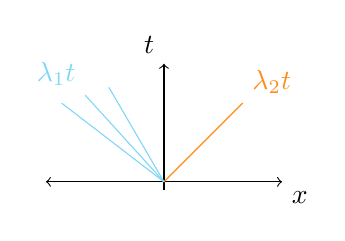
\begin{tikzpicture}
% coord.
\draw[<->] (-1.5,0) -- (1.5,0) node[anchor= north west] {$x$};
\draw[->] (0,-0.1) -- (0,1.5) node[anchor=south east] {$t$};
% contact disc
\draw[color=orange!90!white] (0,0) -- (1,1) node[anchor= south west] {$\lambda_2 t$};
% rarefaction
\draw[color=cyan!50!white] (0,0) -- (-1.3,1);
\draw[color=cyan!50!white] (0,0) -- (-1,1.1) node[anchor= south east] {$\lambda_1 t$};
\draw[color=cyan!50!white] (0,0) -- (-0.7,1.2);
\end{tikzpicture}
\caption{Slow rarefaction (blue) followed by a contact discontinuity (orange).}
\label{Fig:SolRPRarefDiscCongestedPhase}
\end{minipage}
\quad \quad
\begin{minipage}{.3\textwidth}
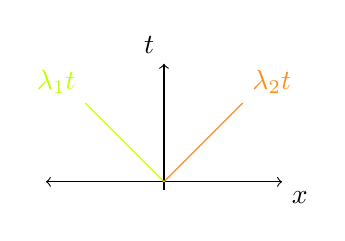
\begin{tikzpicture}
\draw[<->] (-1.5,0) -- (1.5,0) node[anchor= north west] {$x$};
\draw[->] (0,-0.1) -- (0,1.5) node[anchor=south east] {$t$};
\draw[color=orange!90!white] (0,0) -- (1,1) node[anchor= south west] {$\lambda_2 t$};
\draw[color=lime] (0,0) -- (-1,1) node[anchor= south east] {$\lambda_1 t$};
\end{tikzpicture}
\caption{Slow shock (green) followed by a contact discontinuity (orange).}
\label{Fig:SolRPShockDiskCongestedPhase}
\end{minipage}
\quad 
\begin{minipage}{.3\textwidth}
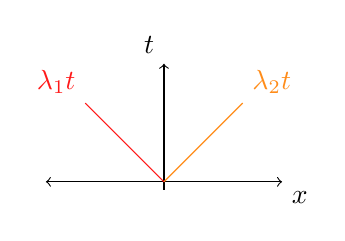
\begin{tikzpicture}
\draw[<->] (-1.5,0) -- (1.5,0) node[anchor= north west] {$x$};
\draw[->] (0,-0.1) -- (0,1.5) node[anchor=south east] {$t$};
\draw[color=orange!90!white] (0,0) -- (1,1) node[anchor= south west] {$\lambda_2 t$};
\draw[color=red!90!white] (0,0) -- (-1,1) node[anchor= south east] {$\lambda_1 t$};
\end{tikzpicture}
\caption{Contact discontinuity followed by a contact discontinuity, $q_l = Q$.}
\label{Fig:SolRPDiscCongestedPhase}
\end{minipage}